\section{寄存器描述}
\regover{
{\hyperref[i2s-i2s-config]{i2s\_config}}&I2S configuration
\\
\hline
{\hyperref[i2s-i2s-int-sts]{i2s\_int\_sts}}&I2S interrupt status
\\
\hline
{\hyperref[i2s-i2s-bclk-config]{i2s\_bclk\_config}}&I2S clock configuration
\\
\hline
{\hyperref[i2s-i2s-fifo-config-0]{i2s\_fifo\_config\_0}}&I2S FIFO configuration0
\\
\hline
{\hyperref[i2s-i2s-fifo-config-1]{i2s\_fifo\_config\_1}}&I2S DMA FIFO configuration
\\
\hline
{\hyperref[i2s-i2s-fifo-wdata]{i2s\_fifo\_wdata}}&I2S FIFO write data
\\
\hline
{\hyperref[i2s-i2s-fifo-rdata]{i2s\_fifo\_rdata}}&I2S FIFO read data
\\
\hline
{\hyperref[i2s-i2s-io-config]{i2s\_io\_config}}&I2S IO configuration
\\
\hline
}

\subsection{i2s\_config}
\label{i2s-i2s-config}
地址:0x4000aa00
 \begin{figure}[H]
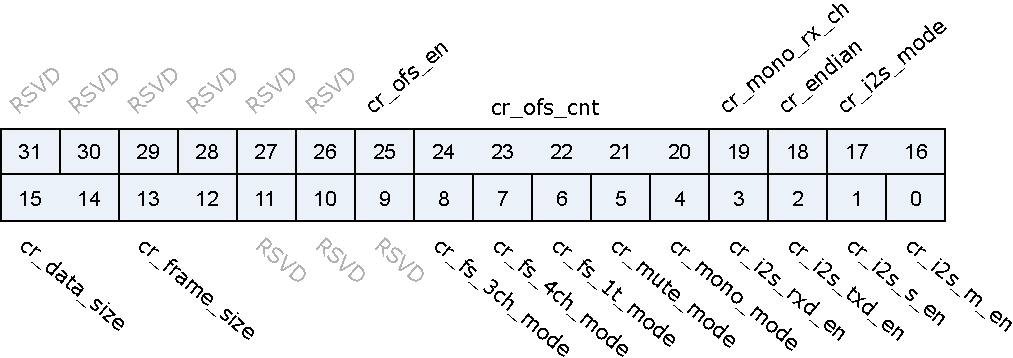
\includegraphics{i2s_i2s_config.pdf}
\end{figure}

\regdes{31:26&RSVD& & & \\\hline
25&cr\_ofs\_en&r/w&1'b0&Offset enable \par 1'b0: Disabled, 1'b1: Enabled
\\\hline
24:20&cr\_ofs\_cnt&r/w&5'd0&Offset cycle count (unit: cycle of I2S BCLK) \par 5'd0: 1 cycle \par 5'd1: 2 cycles \par …
\\\hline
19&cr\_mono\_rx\_ch&r/w&1'b0&RX mono mode channel select signal \par 1'b0: L-channel \par 1'b1: R-channel
\\\hline
18&cr\_endian&r/w&1'b0&Data endian (bit reverse) \par 1'b0: MSB goes out first, 1'b1: LSB goes out first
\\\hline
17:16&cr\_i2s\_mode&r/w&2'd0&2'd0: Left-Justified, 2'd1: Right-Justified, 2'd2: DSP, 2'd3: Reserved\\\hline
15:14&cr\_data\_size&r/w&2'd1&Data bit width of each channel \par 2'd0: 8, 2'd1: 16, 2'd2: 24, 2'd3: 32 (bits)
\\\hline
13:12&cr\_frame\_size&r/w&2'd1&Frame size of each channel \par 2'd0: 8, 2'd1: 16, 2'd2: 24, 2'd3: 32 (cycles)
\\\hline
11:9&RSVD& & & \\\hline
8&cr\_fs\_3ch\_mode&r/w&1'b0&1'b0: FS 2-channel mode, 1'b1: FS 3-channel mode (DSP mode only) \par Note: cr\_fs\_3ch\_mode \& cr\_fs\_4ch\_mode should NOT be enabled at the same time \par Note: cr\_mono\_mode \& cr\_fifo\_lr\_merge will be invalid in 3-channel mode \par Note: When 3-channel mode is enabled, frame\_size must equal data\_size
\\\hline
7&cr\_fs\_4ch\_mode&r/w&1'b0&1'b0: FS 2-channel mode, 1'b1: FS 4-channel mode (DSP mode only) \par Note: cr\_fs\_3ch\_mode \& cr\_fs\_4ch\_mode should NOT be enabled at the same time \par Note: When 4-channel mode is enabled, frame\_size must equal data\_size
\\\hline
6&cr\_fs\_1t\_mode&r/w&1'b0&1'b0: FS high/low is even, 1'b1: FS only asserts for 1 cycle\\\hline
5&cr\_mute\_mode&r/w&1'b0&1'b0: Normal mode, 1'b1: Mute mode\\\hline
4&cr\_mono\_mode&r/w&1'b0&1'b0: Stereo mode, 1'b1: Mono mode \par Note: csr\_mono\_mode \& csr\_fifo\_lr\_merge should NOT be enabled at the same time
\\\hline
3&cr\_i2s\_rxd\_en&r/w&1'b0&Enable signal of I2S RXD signal\\\hline
2&cr\_i2s\_txd\_en&r/w&1'b0&Enable signal of I2S TXD signal\\\hline
1&cr\_i2s\_s\_en&r/w&1'b0&Enable signal of I2S Slave function, cannot enable both csr\_i2s\_m\_en \& csr\_i2s\_s\_en\\\hline
0&cr\_i2s\_m\_en&r/w&1'b0&Enable signal of I2S Master function, cannot enable both csr\_i2s\_m\_en \& csr\_i2s\_s\_en\\\hline

}
\subsection{i2s\_int\_sts}
\label{i2s-i2s-int-sts}
地址:0x4000aa04
 \begin{figure}[H]
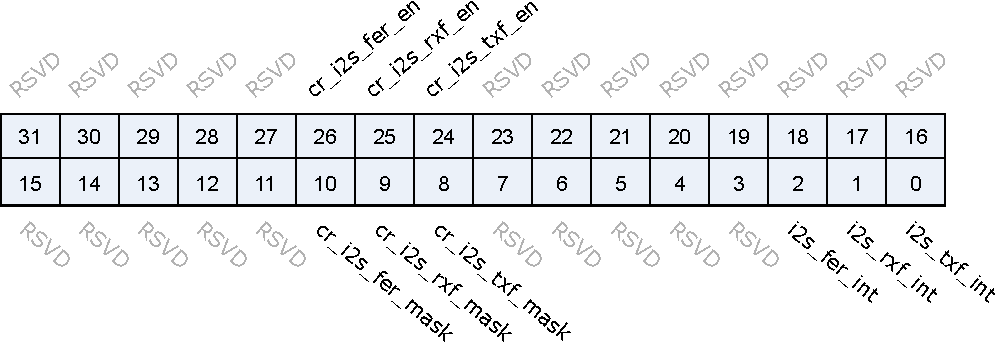
\includegraphics{i2s_i2s_int_sts.pdf}
\end{figure}

\regdes{31:27&RSVD& & & \\\hline
26&cr\_i2s\_fer\_en&r/w&1'b1&Interrupt enable of i2s\_fer\_int\\\hline
25&cr\_i2s\_rxf\_en&r/w&1'b1&Interrupt enable of i2s\_rxf\_int\\\hline
24&cr\_i2s\_txf\_en&r/w&1'b1&Interrupt enable of i2s\_txf\_int\\\hline
23:11&RSVD& & & \\\hline
10&cr\_i2s\_fer\_mask&r/w&1'b1&Interrupt mask of i2s\_fer\_int\\\hline
9&cr\_i2s\_rxf\_mask&r/w&1'b1&Interrupt mask of i2s\_rxf\_int\\\hline
8&cr\_i2s\_txf\_mask&r/w&1'b1&Interrupt mask of i2s\_txf\_int\\\hline
7:3&RSVD& & & \\\hline
2&i2s\_fer\_int&r&1'b0&I2S TX/RX FIFO error interrupt, auto-cleared when FIFO overflow/underflow error flag is cleared\\\hline
1&i2s\_rxf\_int&r&1'b0&I2S RX FIFO ready (rx\_fifo\_cnt > rx\_fifo\_th) interrupt, auto-cleared when data is popped\\\hline
0&i2s\_txf\_int&r&1'b0&I2S TX FIFO ready (tx\_fifo\_cnt > tx\_fifo\_th) interrupt, auto-cleared when data is pushed\\\hline

}
\subsection{i2s\_bclk\_config}
\label{i2s-i2s-bclk-config}
地址:0x4000aa10
 \begin{figure}[H]
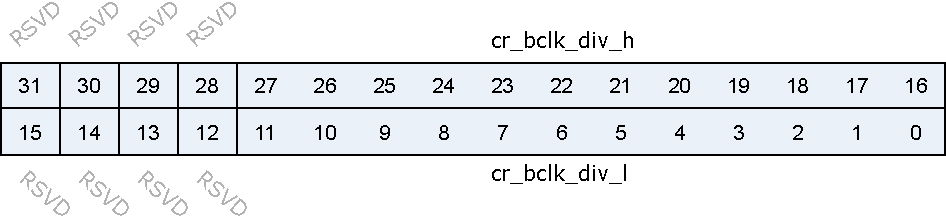
\includegraphics{i2s_i2s_bclk_config.pdf}
\end{figure}

\regdes{31:28&RSVD& & & \\\hline
27:16&cr\_bclk\_div\_h&r/w&12'd1&I2S BCLK active high period (unit: cycle of i2s\_clk)\\\hline
15:12&RSVD& & & \\\hline
11:0&cr\_bclk\_div\_l&r/w&12'd1&I2S BCLK active low period (unit: cycle of i2s\_clk)\\\hline

}
\subsection{i2s\_fifo\_config\_0}
\label{i2s-i2s-fifo-config-0}
地址:0x4000aa80
 \begin{figure}[H]
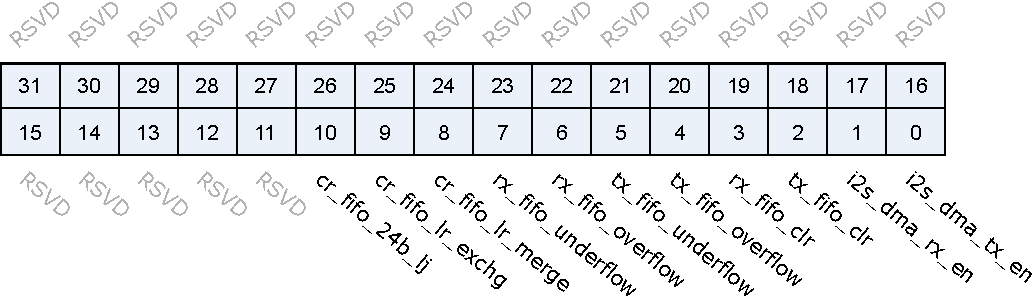
\includegraphics{i2s_i2s_fifo_config_0.pdf}
\end{figure}

\regdes{31:11&RSVD& & & \\\hline
10&cr\_fifo\_24b\_lj&r/w&1'b0&FIFO 24-bit data left-justified mode \par 1'b0: Right-justified, {8'h0, data[23:0]} \par 1'b1: Left-justified, {data[23:0], 8'h0} \par Note: Valid only when cr\_data\_size = 2'd2 (24-bit)
\\\hline
9&cr\_fifo\_lr\_exchg&r/w&1'b0&The position of L/R channel data within each entry is exchanged if this bit is enabled \par Can only be enabled if data size is 8 or 16 bits and csr\_fifo\_lr\_merge is enabled
\\\hline
8&cr\_fifo\_lr\_merge&r/w&1'b0&Each FIFO entry contains both L/R channel data if this bit is enabled \par Can only be enabled if data size is 8 or 16 bits \par Note: cr\_fifo\_lr\_merge \&cr\_mono\_mode should NOT be enabled at the same time \par Note: cr\_fifo\_lr\_merge \&cr\_fifo\_l\_shift should NOT be enabled at the same time
\\\hline
7&rx\_fifo\_underflow&r&1'b0&Underflow flag of RX FIFO, can be cleared by rx\_fifo\_clr\\\hline
6&rx\_fifo\_overflow&r&1'b0&Overflow flag of RX FIFO, can be cleared by rx\_fifo\_clr\\\hline
5&tx\_fifo\_underflow&r&1'b0&Underflow flag of TX FIFO, can be cleared by tx\_fifo\_clr\\\hline
4&tx\_fifo\_overflow&r&1'b0&Overflow flag of TX FIFO, can be cleared by tx\_fifo\_clr\\\hline
3&rx\_fifo\_clr&w1c&1'b0&Clear signal of RX FIFO\\\hline
2&tx\_fifo\_clr&w1c&1'b0&Clear signal of TX FIFO\\\hline
1&i2s\_dma\_rx\_en&r/w&1'b0&Enable signal of dma\_rx\_req/ack interface\\\hline
0&i2s\_dma\_tx\_en&r/w&1'b0&Enable signal of dma\_tx\_req/ack interface\\\hline

}
\subsection{i2s\_fifo\_config\_1}
\label{i2s-i2s-fifo-config-1}
地址:0x4000aa84
 \begin{figure}[H]
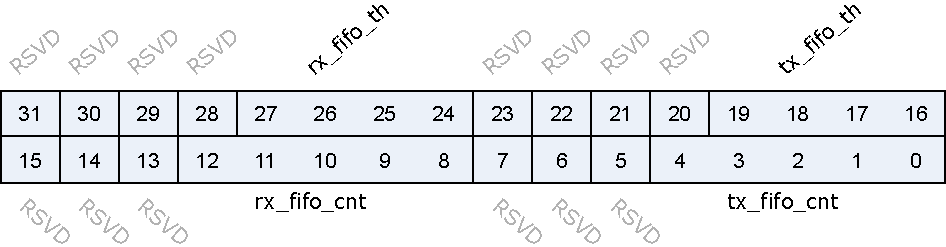
\includegraphics{i2s_i2s_fifo_config_1.pdf}
\end{figure}

\regdes{31:28&RSVD& & & \\\hline
27:24&rx\_fifo\_th&r/w&4'd0&RX FIFO threshold, dma\_rx\_req will not be asserted if tx\_fifo\_cnt is less than this value\\\hline
23:20&RSVD& & & \\\hline
19:16&tx\_fifo\_th&r/w&4'd0&TX FIFO threshold, dma\_tx\_req will not be asserted if tx\_fifo\_cnt is less than this value\\\hline
15:13&RSVD& & & \\\hline
12:8&rx\_fifo\_cnt&r&5'd0&RX FIFO available count\\\hline
7:5&RSVD& & & \\\hline
4:0&tx\_fifo\_cnt&r&5'd16&TX FIFO available count\\\hline

}
\subsection{i2s\_fifo\_wdata}
\label{i2s-i2s-fifo-wdata}
地址:0x4000aa88
 \begin{figure}[H]
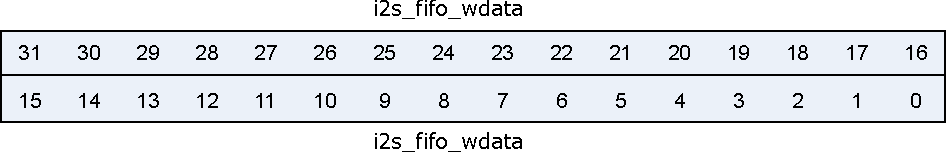
\includegraphics{i2s_i2s_fifo_wdata.pdf}
\end{figure}

\regdes{31:0&i2s\_fifo\_wdata&w&x&\\\hline

}
\subsection{i2s\_fifo\_rdata}
\label{i2s-i2s-fifo-rdata}
地址:0x4000aa8c
 \begin{figure}[H]
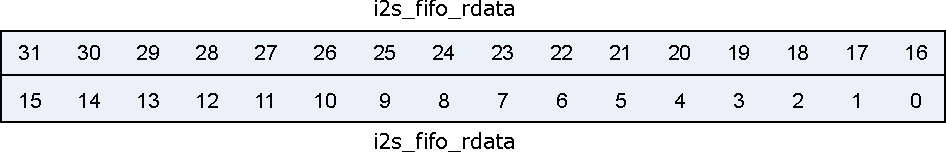
\includegraphics{i2s_i2s_fifo_rdata.pdf}
\end{figure}

\regdes{31:0&i2s\_fifo\_rdata&r&32'h0&\\\hline

}
\subsection{i2s\_io\_config}
\label{i2s-i2s-io-config}
地址:0x4000aafc
 \begin{figure}[H]
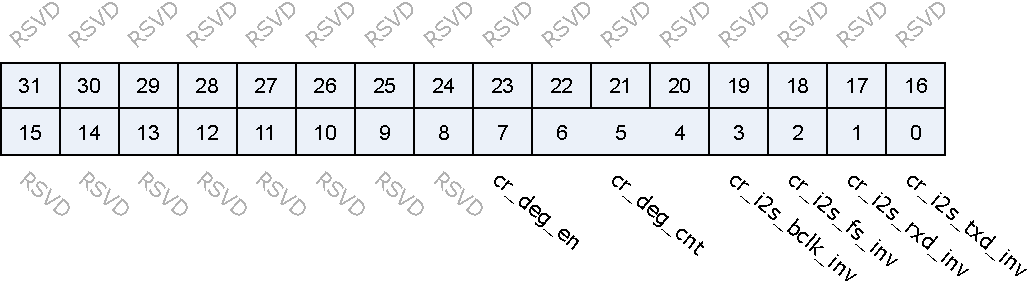
\includegraphics{i2s_i2s_io_config.pdf}
\end{figure}

\regdes{31:8&RSVD& & & \\\hline
7&cr\_deg\_en&r/w&1'b0&Deglitch enable (for all th input pins) \par 1'b0: Disabled, 1'b1: Enabled
\\\hline
6:4&cr\_deg\_cnt&r/w&3'd0&Deglitch cycle count (unit: cycle of I2S kernel clock) \par 3'd0: 1 cycle \par 3'd1: 2 cycles \par …
\\\hline
3&cr\_i2s\_bclk\_inv&r/w&1'b0&Inverse BCLK signal \par 0: No inverse, 1: Inverse
\\\hline
2&cr\_i2s\_fs\_inv&r/w&1'b0&Inverse FS signal \par 0: No inverse, 1: Inverse
\\\hline
1&cr\_i2s\_rxd\_inv&r/w&1'b0&Inverse RXD signal \par 0: No inverse, 1: Inverse
\\\hline
0&cr\_i2s\_txd\_inv&r/w&1'b0&Inverse TXD signal \par 0: No inverse, 1: Inverse
\\\hline

}
